\qrchapter{https://forgottenpillar.com/rsc/en-fp-chapter14}{Adventist pioneers and the Trinity doctrine}


\qrchapter{https://forgottenpillar.com/rsc/en-fp-chapter14}{رواد الأدفنتست وعقيدة الثالوث}


Sister White wrote that early Adventist pioneers \egwinline{are to bear their testimony as to what constitutes the truth for this time}[Lt329-1905.18; 1905][https://egwwritings.org/read?panels=p8455.24] because \egwinline{they have learned to avoid errors and dangers, and are they not then competent to give wise counsel}[7T 287.3; 1902][https://egwwritings.org/read?panels=p117.1637]? In their writings, we see their unanimous views regarding the \emcap{personality of God}, and that they have avoided the Trinitarian error. There is much to write about this topic because the Adventist pioneers left a lot of material dealing directly or indirectly with the doctrine of Trinity. But we will look at some of the testimonies from James White and brother Loughborough because we have read some of their articles on the \emcap{personality of God}. Also, we will compare their testimony with the Spirit of Prophecy as we have done so far.


كتبت الأخت وايت أن رواد الأدفنتست الأوائل \egwinline{عليهم أن يقدموا شهادتهم حول ما يشكل الحق لهذا الوقت}[Lt329-1905.18; 1905][https://egwwritings.org/read?panels=p8455.24] لأنهم \egwinline{تعلموا تجنب الأخطاء والمخاطر، أفليسوا إذن مؤهلين لتقديم المشورة الحكيمة}[7T 287.3; 1902][https://egwwritings.org/read?panels=p117.1637]؟ في كتاباتهم، نرى آراءهم المتفقة بخصوص \emcap{شخصانية الله}، وأنهم تجنبوا خطأ الثالوث. هناك الكثير للكتابة عن هذا الموضوع لأن رواد الأدفنتست تركوا الكثير من المواد التي تتعامل بشكل مباشر أو غير مباشر مع عقيدة الثالوث. لكننا سننظر إلى بعض الشهادات من جيمس وايت والأخ لوبورو لأننا قرأنا بعض مقالاتهم عن \emcap{شخصانية الله}. أيضًا، سنقارن شهادتهم مع روح النبوة كما فعلنا حتى الآن.


James White, in the Review and Herald, listed \others{some of \textbf{the popular fables} of the age}”, saying: “\others{Here we might mention \textbf{the Trinity, which \underline{does away the personality of God, and of his Son Jesus Christ,} }and of sprinkling or pouring instead of being ‘buried with Christ in baptism,’ ‘planted in the likeness of his death:’ but we pass from these \textbf{fables }to notice one that is held sacred by nearly all professed Christians, both Catholic and Protestant. It is, the change of the Sabbath of the fourth commandment from the seventh to the first day of the week.}[James S. White, Review \& Herald, December 11, 1855, p. 85.15][http://documents.adventistarchives.org/Periodicals/RH/RH18551211-V07-11.pdf]


جيمس وايت، في مجلة ريفيو آند هيرالد، ذكر \others{بعض \textbf{الخرافات الشائعة} في العصر}”، قائلاً: “\others{هنا يمكننا أن نذكر \textbf{الثالوث، الذي \underline{يلغي شخصانية الله، وابنه يسوع المسيح،} }والرش أو السكب بدلاً من أن نكون ‘مدفونين مع المسيح في المعمودية،‘ ‘مغروسين في شبه موته:’ لكننا ننتقل من هذه \textbf{الخرافات }لنلاحظ واحدة يعتبرها مقدسة تقريبًا جميع المسيحيين المعترفين، سواء الكاثوليك والبروتستانت. إنها تغيير سبت الوصية الرابعة من اليوم السابع إلى اليوم الأول من الأسبوع.}[James S. White, Review \& Herald, December 11, 1855, p. 85.15][http://documents.adventistarchives.org/Periodicals/RH/RH18551211-V07-11.pdf]


What does James White mean when he says that the Trinity \others{does away with the personality of God, and of his Son Jesus Christ}? In Day Star, he wrote:


ماذا يقصد جيمس وايت عندما يقول إن الثالوث \others{يلغي شخصانية الله، وابنه يسوع المسيح}؟ في داي ستار، كتب:


\others{…a certain class who \textbf{deny the only Lord God and our Lord Jesus Christ}. This class can be no other than those who \textbf{spiritualize away the existence of the Father and the Son}, \textbf{as \underline{two distinct}, \underline{literal}, \underline{tangible persons}}, also a literal Holy city and throne of David… The way spiritualizers this way have disposed of or \textbf{denied the only Lord God and our Lord Jesus Christ is first using \underline{the old unscriptural trinitarian creed}}, viz, that Jesus Christ is the eternal God, though they have not one passage to support it, while we have plain scripture testimony in abundance \textbf{that He is the Son of the eternal God.}}[James White, Day Star, Jan 24, 1846][https://m.egwwritings.org/en/book/741.25\#27]


\others{...فئة معينة \textbf{تنكر الرب الإله الوحيد وربنا يسوع المسيح}. هذه الفئة لا يمكن أن تكون سوى أولئك الذين \textbf{يروحنون وجود الآب والابن}، \textbf{كـ \underline{شخصين} \underline{حرفيين}، \underline{ملموسين} \underline{متميزين}}، وكذلك مدينة مقدسة حرفية وعرش داود... الطريقة التي تخلص بها الروحانيون من أو \textbf{أنكروا الرب الإله الوحيد وربنا يسوع المسيح هي أولاً باستخدام \underline{عقيدة الثالوث القديمة غير الكتابية}}، أي أن يسوع المسيح هو الله الأزلي، مع أنه ليس لديهم نص واحد يدعم ذلك، بينما لدينا شهادة كتابية واضحة بوفرة \textbf{أنه ابن الله الأزلي.}}[James White, Day Star, Jan 24, 1846][https://m.egwwritings.org/en/book/741.25\#27]


Doing away with the personality of God and His Son is accomplished by denying Them as two distinct, literal, and tangible persons. The doctrine on the personality of God teaches that the Father has a literal, \textit{tangible} person.


إلغاء شخصانية الله وابنه يتم من خلال إنكارهما كشخصين متميزين، حرفيين، وملموسين. تعلّم عقيدة شخصانية الله أن الآب له شخص حرفي، \textit{ملموس}.


In the Adventist Review and Sabbath Herald article from April 4, 1854, James White listed 10 points of \textit{Catholic reasons for keeping Sunday}”, where he said that the Sunday \others{is a day dedicated by the apostles to \textbf{the honor of the most Holy Trinity}}[The Advent Review, and Sabbath Herald, vol. 5 April 4, 1854, p. 86][https://egwwritings.org/read?panels=p1643.2867]. Here we also see the harmony between J. B. Frisbie and James White in their view that the Sabbath is dedicated to the biblical God expressed in the first point of the \emcap{Fundamental Principles}, and Sunday is dedicated to the trinity God. The main problem with the Trinity doctrine is that it \others{does away the personality of God, and of his Son Jesus Christ}. In Life Incidents, he wrote more about why this is so.


في مقال مجلة أدفنتست ريفيو آند سباث هيرالد بتاريخ 4 أبريل 1854، ذكر جيمس وايت 10 نقاط من \textit{الأسباب الكاثوليكية للحفاظ على يوم الأحد}”، حيث قال إن الأحد \others{هو يوم كرسه الرسل \textbf{لتكريم الثالوث الأقدس}}[The Advent Review, and Sabbath Herald, vol. 5 April 4, 1854, p. 86][https://egwwritings.org/read?panels=p1643.2867]. هنا نرى أيضًا التناغم بين ج. ب. فريسبي وجيمس وايت في رؤيتهم أن السبت مكرس لله الكتابي المعبر عنه في النقطة الأولى من \emcap{المبادئ الأساسية}، والأحد مكرس لإله الثالوث. المشكلة الرئيسية مع عقيدة الثالوث هي أنها \others{تلغي شخصانية الله، وابنه يسوع المسيح}. في كتاب “حوادث الحياة”، كتب المزيد عن سبب ذلك.


\others{\textbf{Jesus prayed that his disciples might be one as he was \underline{one with his Father}}. \textbf{This prayer did not contemplate one disciple with twelve heads, but twelve disciples, made one in object and effort in the cause of their Master}. \textbf{\underline{Neither are the Father and the Son parts of the ‘three-one God.}}’\footnote{The same quotation is found in James White’s book “\textit{The Law and the Gospel}” with one difference. He states, “\textit{Neither are the Father and the Son parts of \underline{one being}}”; in “\textit{Life Incidents}”, he wrote “parts of the ‘\underline{three-one God}’”. See \href{https://egwwritings.org/?ref=en_LAGO.1.2&para=1492.10}{James S. White, The Law and the Gospel p. 1.2}.} \textbf{\underline{They are two distinct beings}}, \textbf{yet one in the design and accomplishment of redemption}. The redeemed, from the first who shares in the great redemption, to the last, all ascribe the honour, and glory, and praise, of their salvation, to \textbf{both God and the Lamb}.}[James S. White, Life Incidents, p.343.2][https://egwwritings.org/read?panels=p1462.1743]


\others{\textbf{صلى يسوع أن يكون تلاميذه واحدًا كما كان هو \underline{واحدًا مع أبيه}}. \textbf{هذه الصلاة لم تتصور تلميذًا واحدًا بإثني عشر رأسًا، بل إثني عشر تلميذًا، صاروا واحدًا في الهدف والجهد في قضية معلمهم}. \textbf{\underline{كما أن الآب والابن ليسا جزءين من ‘الإله الثلاثي الواحد.}}’\footnote{نفس الاقتباس موجود في كتاب جيمس وايت “\textit{الناموس والإنجيل}” مع اختلاف واحد. يقول، “\textit{كما أن الآب والابن ليسا جزءين من \underline{كائن واحد}}”; في “\textit{حوادث الحياة}”، كتب “جزءين من ‘\underline{الإله الثلاثي الواحد}’“. انظر \href{https://egwwritings.org/?ref=en_LAGO.1.2&para=1492.10}{James S. White, The Law and the Gospel p. 1.2}.} \textbf{\underline{إنهما كائنان متميزان}}, \textbf{لكنهما واحد في تصميم وإنجاز الفداء}. المفديون، من أول من يشارك في الفداء العظيم، إلى الأخير، جميعهم ينسبون الإكرام، والمجد، والتسبيح، لخلاصهم، \textbf{لله والحمل معًا}.}[James S. White, Life Incidents, p.343.2][https://egwwritings.org/read?panels=p1462.1743]


Sister White wrote similarly regarding Christ’s prayer:


كتبت الأخت وايت بطريقة مماثلة بخصوص صلاة المسيح:


\egw{The burden of that prayer was that His disciples might be \textbf{one as He was one with the Father}; the oneness so close that, \textbf{although \underline{two distinct beings}}, there was \textbf{perfect unity of spirit, purpose, and action}. The mind of the Father was the mind of the Son.}[Lt1-1882.1; 1882][https://egwwritings.org/read?panels=p4120.5]


\egw{كان عبء تلك الصلاة أن يكون تلاميذه \textbf{واحدًا كما كان هو واحدًا مع الآب}؛ وحدة وثيقة لدرجة أنه، \textbf{رغم كونهما \underline{كائنين متميزين}}، كانت هناك \textbf{وحدة تامة في الروح والهدف والعمل}. عقل الآب كان عقل الابن.}[Lt1-1882.1; 1882][https://egwwritings.org/read?panels=p4120.5]


\egw{\textbf{The unity that exists between Christ and His disciples \underline{does not destroy the personality of either}}. They are one in purpose, in mind, in character, \textbf{but \underline{not in person}}. \textbf{It is thus that God and Christ are one}.}[MH, 421 422; 1905][https://egwwritings.org/read?panels=p135.2177]


\egw{\textbf{إن الوحدة الموجودة بين المسيح وتلاميذه \underline{لا تدمر شخصانية أي منهما}}. هم واحد في الهدف، في الفكر، في الشخصية، \textbf{ولكن \underline{ليس في الشخص}}. \textbf{هكذا الله والمسيح واحد}.}[MH, 421 422; 1905][https://egwwritings.org/read?panels=p135.2177]


The Father and the Son do not comprise one person nor being. The Father and the Son are one, just as Christ and His disciples are one—one in spirit, purpose, mind, and character.


الآب والابن لا يشكلان شخصًا واحدًا ولا كائنًا واحدًا. الآب والابن واحد، تمامًا كما أن المسيح وتلاميذه واحد - واحد في الروح، والهدف، والفكر، والشخصية.


Many Adventist trinitarian scholars charge James White and other early pioneers for arianism or semi-arianism, claiming that they made Christ inferior to the Father. This is not true. Let us read the testimony of James White on this matter.


يتهم العديد من علماء الأدفنتست المؤمنين بالثالوث جيمس وايت وغيره من الرواد الأوائل بالآريوسية أو شبه الآريوسية، مدعين أنهم جعلوا المسيح أدنى من الآب. هذا غير صحيح. دعونا نقرأ شهادة جيمس وايت حول هذه المسألة.


\others{Paul affirms of \textbf{the Son of God that he was in the form of God}, and that \textbf{\underline{he was equal with God}}. ‘\textbf{Who being in the form of God thought it not robbery to be \underline{equal with God}}.’ Phil. 2:6. The reason why it is not robbery for the Son \textbf{to be equal with the Father is the fact that he is equal}. If the Son is not equal with the Father, then it is robbery for him to rank himself with the Father.}


\others{يؤكد بولس عن \textbf{ابن الله أنه كان في صورة الله}، وأنه \textbf{\underline{كان مساويًا لله}}. ‘\textbf{الذي إذ كان في صورة الله، لم يحسب خلسة أن يكون \underline{مساويًا لله}}.’ فيلبي 2:6. السبب في أنه ليس خلسة للابن \textbf{أن يكون مساويًا للآب هو حقيقة أنه مساوٍ}. إذا لم يكن الابن مساويًا للآب، فسيكون خلسة أن يضع نفسه في مرتبة الآب.}


\othersnogap{\textbf{\underline{The inexplicable trinity that makes the godhead three in one and one in three, is bad enough}}; \textbf{but that ultra Unitarianism that makes Christ inferior to the Father is worse}. Did God say to an inferior, Let us make man in our image?’}[James S. White, The Advent Review and Sabbath Herald, November 29, 1877, p. 171][https://documents.adventistarchives.org/Periodicals/RH/RH18771129-V50-22.pdf]


\othersnogap{\textbf{\underline{الثالوث الذي لا يمكن تفسيره والذي يجعل اللاهوت ثلاثة في واحد وواحد في ثلاثة، هو سيء بما فيه الكفاية}}؛ \textbf{لكن تلك الوحدانية المتطرفة التي تجعل المسيح أدنى من الآب هي أسوأ}. هل قال الله لمن هو أدنى منه، لنصنع الإنسان على صورتنا؟‘}[James S. White, The Advent Review and Sabbath Herald, November 29, 1877, p. 171][https://documents.adventistarchives.org/Periodicals/RH/RH18771129-V50-22.pdf]


The problem of the Adventist trinitarian scholars lies in that they themselves cannot completely explain Christ’s divinity other than through the Trinitarian paradigm. Adventist pioneers did believe in Christ’s full divinity but they rejected the Trinity because it destroys the \emcap{personality of God}. \others{The inexplicable trinity that makes the godhead three in one and one in three, \textbf{is bad enough}}. Below is another statement from James White where he compared Seventh-day Adventist with Seventh-day Baptist belief. Seventh-day Adventists did not believe in the Trinity unlike Seventh-day Baptists. James White mentioned that, regarding the divinity of Christ, Seventh-day Adventists hold so nearly with the trinitarian Seventh-day Baptists that they apprehend no trial there.


تكمن مشكلة علماء الأدفنتست المؤمنين بالثالوث في أنهم أنفسهم لا يستطيعون شرح ألوهية المسيح بشكل كامل إلا من خلال نموذج الثالوث. آمن رواد الأدفنتست بألوهية المسيح الكاملة لكنهم رفضوا الثالوث لأنه يدمر \emcap{شخصانية الله}. \others{الثالوث الذي لا يمكن تفسيره والذي يجعل اللاهوت ثلاثة في واحد وواحد في ثلاثة، \textbf{هو سيء بما فيه الكفاية}}. فيما يلي بيان آخر من جيمس وايت حيث قارن بين معتقد الأدفنتست السبتيين ومعتقد المعمدانيين السبتيين. لم يؤمن الأدفنتست السبتيون بالثالوث على عكس المعمدانيين السبتيين. ذكر جيمس وايت أنه فيما يتعلق بألوهية المسيح، يتمسك الأدفنتست السبتيون بما يقارب جدًا معتقد المعمدانيين السبتيين المؤمنين بالثالوث لدرجة أنهم لا يتوقعون أي خلاف هناك.


\others{\textbf{The principal difference between the two bodies is the immortality question}. \textbf{The S. D. Adventists hold \underline{the divinity of Christ so nearly with the trinitarian}, that we apprehend no trial here}. And as the practical application of the subject of the Gifts of the Spirit to our people and to our work is better understood by our S. D. Baptist brethren, they manifest less concern for us on this account.}[James S. White, The Advent Review and Sabbath Herald, October 12, 1876, p. 116][https://documents.adventistarchives.org/Periodicals/RH/RH18761012-V48-15.pdf]


\others{\textbf{الاختلاف الرئيسي بين الطائفتين هو مسألة الخلود}. \textbf{يتمسك الأدفنتست السبتيون \underline{بألوهية المسيح بشكل قريب جدًا من المؤمنين بالثالوث}، لدرجة أننا لا نتوقع أي خلاف هنا}. وبما أن التطبيق العملي لموضوع مواهب الروح على شعبنا وعلى عملنا مفهوم بشكل أفضل من قبل إخواننا المعمدانيين السبتيين، فإنهم يظهرون قلقًا أقل علينا في هذا الصدد.}[James S. White, The Advent Review and Sabbath Herald, October 12, 1876, p. 116][https://documents.adventistarchives.org/Periodicals/RH/RH18761012-V48-15.pdf]


This evidence should raise questions to each Adventist trinitarian scholar. How could it be that the Adventist pioneers adhere to the divinity of Christ as trinitarians did, yet rejected the Trinity doctrine? In which way was Christ fully divine, if He was not part of an amalgamated three-in-one God? The answer is simple and completely Biblical. Christ is fully divine, just as His Father, because He was begotten in the express image of the Father’s person; thus, He inherited complete divine nature from His Father.


ينبغي لهذا الدليل أن يثير أسئلة لكل عالم أدفنتستي مؤمن بالثالوث. كيف يمكن أن يتمسك رواد الأدفنتست بألوهية المسيح كما فعل المؤمنون بالثالوث، ومع ذلك رفضوا عقيدة الثالوث؟ بأي طريقة كان المسيح إلهيًا بالكامل، إذا لم يكن جزءًا من إله مدمج ثلاثة في واحد؟ الإجابة بسيطة وكتابية تمامًا. المسيح إلهي بالكامل، تمامًا مثل أبيه، لأنه وُلد على صورة جوهر الآب؛ وبالتالي، ورث الطبيعة الإلهية الكاملة من أبيه.


\egw{A complete offering has been made; for ‘God so loved the world, that he gave his only-begotten Son,’—\textbf{not a son by creation}, as were the angels, nor a son by adoption, as is the forgiven sinner, but \textbf{a Son \underline{begotten} in the express image of the Father’s person}, and in all the brightness of his majesty and glory, \textbf{one equal with God} in authority, dignity, and \textbf{divine perfection}. \textbf{In him dwelt all the fullness of the Godhead bodily}.}[ST May 30, 1895, par. 3; 1895][https://egwwritings.org/read?panels=p820.12891]


\egw{لقد قُدمت ذبيحة كاملة؛ لأن ‘الله أحب العالم حتى بذل ابنه الوحيد،‘ - \textbf{ليس ابنًا بالخلق}، كما كانت الملائكة، ولا ابنًا بالتبني، كما هو الخاطئ المغفور له، بل \textbf{ابنًا \underline{مولودًا} على صورة جوهر الآب}، وفي كل بهاء جلاله ومجده، \textbf{مساويًا لله} في السلطة والكرامة \textbf{والكمال الإلهي}. \textbf{فيه يحل كل ملء اللاهوت جسديًا}.}[ST May 30, 1895, par. 3; 1895][https://egwwritings.org/read?panels=p820.12891]


Christ's complete divinity is not based on an amalgamated \emcap{personality of God}, but rather on His Sonship with the Father. The Bible never refers to Christ with the term “\textit{one God}”—only the Father is referred to with the term “\textit{one God}”\footnote{John 17:3; 1. Corinthians 8:6; 1. Timothy 2:5; Ephesians 4:6} \footnote{We study Christ’s complete divinity in-depth  in the second book of the Forgotten Pillar Project - “\textit{Rediscovering the Pillar}”}. Jesus, the Son of God, is fully divine but is not referred to as \others{\textbf{one God}, \textbf{a personal, spiritual being}} in the first point of the \emcap{Fundamental Principles}.


ألوهية المسيح الكاملة لا تستند على \emcap{شخصانية الله} المدمجة، بل على بنوته مع الآب. الكتاب المقدس لا يشير أبدًا إلى المسيح بمصطلح “\textit{إله واحد}” - فقط الآب يُشار إليه بمصطلح “\textit{إله واحد}”\footnote{يوحنا 17:3؛ 1 كورنثوس 8:6؛ 1 تيموثاوس 2:5؛ أفسس 4:6} \footnote{ندرس ألوهية المسيح الكاملة بعمق في الكتاب الثاني من مشروع العمود المنسي - “\textit{إعادة اكتشاف العمود}”}. يسوع، ابن الله، إلهي بالكامل ولكن لا يُشار إليه كـ \others{\textbf{إله واحد}، \textbf{كائن شخصي روحي}} في النقطة الأولى من \emcap{المبادئ الأساسية}.


\egw{The Lord Jesus Christ, the only begotten Son of the Father, \textbf{is truly God in infinity, \underline{but not in personality}}.}[Ms116-1905.19; 1905][https://egwwritings.org/read?panels=p10633.25]


\egw{الرب يسوع المسيح، الابن الوحيد للآب، \textbf{هو حقًا الله في اللانهائية، \underline{ولكن ليس في الشخصانية}}.}[Ms116-1905.19; 1905][https://egwwritings.org/read?panels=p10633.25]


Brother J. N. Loughborough was asked to answer the question, \others{What serious objection is there to the doctrine of the Trinity?}[The question was asked by Brother W. W. Giles and it was sent to James S. White, who forwarded the question to Brother John N. Loughborough.]. As we read his answer, let us try to understand some of the reasons why the early pioneers did not adhere to this doctrine.


طُلب من الأخ ج. ن. لوبورو الإجابة على السؤال، \others{ما هو الاعتراض الجاد على عقيدة الثالوث؟}[تم طرح السؤال من قبل الأخ و. و. جايلز وتم إرساله إلى جيمس س. وايت، الذي أحال السؤال إلى الأخ جون ن. لوبورو.]. بينما نقرأ إجابته، دعونا نحاول فهم بعض الأسباب التي جعلت الرواد الأوائل لا يتمسكون بهذه العقيدة.


\others{There are many objections which we might urge, but on account of our limited space we shall reduce them to the three following: \textbf{1. It is contrary to common sense. 2. It is contrary to scripture. 3. Its origin is Pagan and fabulous.}}


\others{هناك العديد من الاعتراضات التي يمكن أن نقدمها، ولكن بسبب مساحتنا المحدودة سنختصرها إلى الاعتراضات الثلاثة التالية: \textbf{1. إنها مخالفة للمنطق السليم. 2. إنها مخالفة للكتاب المقدس. 3. أصلها وثني وخرافي.}}


\othersnogap{These positions we will remark upon briefly in their order. And 1. \textbf{It is not very consonant with common sense to talk of three being one, and one being three}. \textbf{Or as some express it, calling God ‘the Triune God,’ or ‘the three-one-God.’} \textbf{If Father, Son, and Holy Ghost are each God, it would be three Gods; for three times one is not one, but three}. \textbf{\underline{There is a sense in which they are one, but not one person, as claimed by Trinitarians}}}.


\othersnogap{سنعلق على هذه المواقف باختصار حسب ترتيبها. وأولاً: \textbf{ليس من المنطقي الحديث عن ثلاثة يكونون واحدًا، وواحد يكون ثلاثة}. \textbf{أو كما يعبر البعض، بتسمية الله ‘الإله الثالوثي’ أو ‘الإله الثلاثة في واحد.’} \textbf{إذا كان الآب والابن والروح القدس كل منهم إله، فسيكون ثلاثة آلهة؛ لأن ثلاثة مضروبة في واحد ليست واحدًا، بل ثلاثة}. \textbf{\underline{هناك معنى يكونون فيه واحدًا، ولكن ليس شخصًا واحدًا، كما يدعي المؤمنون بالثالوث}}}.


\othersnogap{2. \textbf{It is contrary to Scripture}. \textbf{Almost any portion of the New Testament we may open which has occasion to speak of the Father and Son, represents them as two distinct persons}. \textbf{\underline{The seventeenth chapter of John is alone sufficient to refute the doctrine of the Trinity}}. \textbf{Over forty times in that one chapter Christ speaks of his Father as a person distinct from himself}. His Father was in heaven and he upon earth. The Father had sent him. Given to him those that believed. He was then to go to the Father.\textbf{ And in this very testimony he shows us in what consists the oneness of the Father and Son}.\textbf{\underline{ It is the same as the oneness of the members of Christ’s church}}. ‘\textbf{That \underline{they} all may be one; \underline{as} thou, Father, art in me, and I in thee, \underline{that they also} may be one in us}; that the world may believe that thou hast sent me. And the \textbf{glory which thou gavest me I have given them}; that \textbf{they may be one}, \textbf{even as we are one.}’ \textbf{Of one heart and one mind}. \textbf{Of one purpose} in all the plan devised for man’s salvation. \textbf{\underline{Read the seventeenth chapter of John, and see if it does not completely upset the doctrine of the Trinity}}.}


\othersnogap{2. \textbf{إنها مخالفة للكتاب المقدس}. \textbf{أي جزء تقريبًا من العهد الجديد يمكننا فتحه والذي يتحدث عن الآب والابن، يمثلهما كشخصين متميزين}. \textbf{\underline{الإصحاح السابع عشر من إنجيل يوحنا وحده كافٍ لدحض عقيدة الثالوث}}. \textbf{أكثر من أربعين مرة في ذلك الإصحاح الواحد يتحدث المسيح عن أبيه كشخص متميز عنه}. كان أبوه في السماء وهو على الأرض. الآب أرسله. أعطاه الذين آمنوا. كان عليه أن يذهب إلى الآب.\textbf{ وفي هذه الشهادة نفسها يبين لنا ما تتكون منه وحدة الآب والابن}.\textbf{\underline{ إنها نفس وحدة أعضاء كنيسة المسيح}}. ‘\textbf{ليكون \underline{الجميع} واحدًا؛ \underline{كما} أنك أنت أيها الآب فيّ، وأنا فيك، \underline{ليكونوا هم أيضًا} واحدًا فينا}؛ ليؤمن العالم أنك أرسلتني. و\textbf{المجد الذي أعطيتني قد أعطيتهم}؛ \textbf{ليكونوا واحدًا}، \textbf{كما نحن واحد.} \textbf{بقلب واحد وفكر واحد}. \textbf{بهدف واحد} في كل الخطة المصممة لخلاص الإنسان. \textbf{\underline{اقرأ الإصحاح السابع عشر من إنجيل يوحنا، وانظر إذا كان لا يقلب عقيدة الثالوث رأسًا على عقب}}.}


\othersnogap{\textbf{To believe that doctrine, when reading the scripture we must believe that God sent himself into the world, died to reconcile the world to himself, raised himself from the dead, ascended to himself in heaven, pleads before himself in heaven to reconcile the world to himself, and is the only mediator between man and himself}. It will not do to substitute the human nature of Christ (according to Trinitarians) as the Mediator; for Clarke says, ‘Human blood can no more appease God than swine’s blood.’ Comment on 2 Samuel 21:10. \textbf{We must believe also that in the garden God prayed to himself, if it were possible, to let the cup pass from himself, and a thousand other \underline{such absurdities}}.}


\othersnogap{\textbf{للإيمان بتلك العقيدة، عند قراءة الكتاب المقدس علينا أن نؤمن أن الله أرسل نفسه إلى العالم، ومات ليصالح العالم مع نفسه، وأقام نفسه من الموت، وصعد إلى نفسه في السماء، ويتوسل أمام نفسه في السماء ليصالح العالم مع نفسه، وهو الوسيط الوحيد بين الإنسان ونفسه}. لن يجدي استبدال الطبيعة البشرية للمسيح (وفقًا للمؤمنين بالثالوث) كوسيط؛ لأن كلارك يقول، ‘الدم البشري لا يمكن أن يرضي الله أكثر من دم الخنزير.’ تعليق على 2 صموئيل 21:10. \textbf{يجب أن نؤمن أيضًا أنه في البستان صلى الله إلى نفسه، إن كان ممكنًا، أن تعبر عنه الكأس، وألف \underline{سخافة} أخرى مثل هذه}.}


\othersnogap{\textbf{Read carefully the following texts, comparing them with the idea that Christ is the Omnipotent, Omnipresent, Supreme, and only self-existent God: John 14:28; 17:3; 3:16; 5:19, 26; 11:15; 20:19; 8:50; 6:38; Mark 13:32; Luke 6:12; 22:69; 24:29; Matthew 3:17; 27:46; Galatians 3:20; 1 John 2:1; Revelation 5:7; Acts 17:31. Also see Matthew 11:25, 27; Luke 1:32; 22:42; John 3:35, 36; 5:19, 21, 22, 23, 25, 26; 6:40; 8:35, 36; 14:13; 1 Corinthians 15:28, etc}.}


\othersnogap{\textbf{اقرأ بعناية النصوص التالية، مقارنة إياها بفكرة أن المسيح هو الإله القدير، الحاضر في كل مكان، الأسمى، والوحيد الموجود بذاته: يوحنا 14:28؛ 17:3؛ 3:16؛ 5:19، 26؛ 11:15؛ 20:19؛ 8:50؛ 6:38؛ مرقس 13:32؛ لوقا 6:12؛ 22:69؛ 24:29؛ متى 3:17؛ 27:46؛ غلاطية 3:20؛ 1 يوحنا 2:1؛ رؤيا 5:7؛ أعمال 17:31. انظر أيضًا متى 11:25، 27؛ لوقا 1:32؛ 22:42؛ يوحنا 3:35، 36؛ 5:19، 21، 22، 23، 25، 26؛ 6:40؛ 8:35، 36؛ 14:13؛ 1 كورنثوس 15:28، إلخ}.}


\othersnogap{\textbf{The word Trinity nowhere occurs in the Scriptures}. \textbf{The principal text supposed to teach it is 1 John 1:7\footnote{J. N. Loughborough made a typo in the original document, he wanted to point out to 1 John 5:7}, which is an interpolation}. Clarke says, ‘\textbf{Out of one hundred and thirteen manuscripts, the text is wanting in one hundred and twelve. It occurs in no MS. before the tenth century. And the first place the text occurs in Greek, is in the Greek translation of the acts of the Council of Lateran, held A. D. 1215}.’ - Comment. on John 1, and remarks at close of chap.}


\othersnogap{\textbf{كلمة الثالوث لا ترد في أي مكان في الكتاب المقدس}. \textbf{النص الرئيسي المفترض أنه يعلّمها هو 1 يوحنا 1:7\footnote{ارتكب ج. ن. لوبورو خطأً مطبعيًا في الوثيقة الأصلية، كان يريد الإشارة إلى 1 يوحنا 5:7}، وهو إضافة مقحمة}. يقول كلارك، ‘\textbf{من بين مائة وثلاثة عشر مخطوطة، النص مفقود في مائة واثنتي عشرة. لا يظهر في أي مخطوطة قبل القرن العاشر. وأول مكان يظهر فيه النص باليونانية، هو في الترجمة اليونانية لأعمال مجلس لاتيران، الذي عُقد عام 1215 م}.’ - تعليق على يوحنا 1، وملاحظات في نهاية الفصل.}


\othersnogap{3. \textbf{Its origin is pagan and fabulous}. Instead of pointing us to scripture for proof of the trinity, we are pointed to the trident of the Persians, with the assertion that by this they designed to teach the idea of a trinity, and if they had the doctrine of the trinity, they must have received it by tradition from the people of God. \textbf{But this is all assumed, for it is certain that the Jewish church held to no such doctrine. Says Mr. Summerbell, ‘A friend of mine who was present in a New York synagogue, asked the Rabbi for an explanation of the \underline{word ’elohim’}. A Trinitarian clergyman who stood by, replied, ‘Why, that has \underline{reference to the three persons in the Trinity},’ when a Jew stepped forward and said he must not mention that word again, or they would have to compel him to leave the house; \underline{for it was not permitted to mention the name of any strange god in the synagogue}.’}\footnote{Discussion between Summerbell and Flood on Trinity, p.38.} Milman says the idea of the Trident is fabulous. (Hist. Christianity, p.34.)}


\othersnogap{3. \textbf{أصلها وثني وخرافي}. بدلاً من توجيهنا إلى الكتاب المقدس لإثبات الثالوث، يتم توجيهنا إلى الرمح الثلاثي الشعب للفرس، مع التأكيد أنهم قصدوا بهذا تعليم فكرة الثالوث، وإذا كانت لديهم عقيدة الثالوث، فلا بد أنهم تلقوها بالتقليد من شعب الله. \textbf{لكن هذا كله افتراض، لأنه من المؤكد أن الكنيسة اليهودية لم تتمسك بمثل هذه العقيدة. يقول السيد سمربل، ‘صديق لي كان حاضرًا في كنيس يهودي في نيويورك، سأل الحاخام عن تفسير \underline{كلمة ‘إلوهيم’}. فرد رجل دين مؤمن بالثالوث كان واقفًا بالقرب، ‘لماذا، هذا \underline{يشير إلى الأشخاص الثلاثة في الثالوث}’، عندها تقدم يهودي وقال إنه يجب ألا يذكر تلك الكلمة مرة أخرى، وإلا سيضطرون إلى إجباره على مغادرة المكان؛ \underline{لأنه لم يكن مسموحًا بذكر اسم أي إله غريب في الكنيس}.’}\footnote{مناقشة بين سمربل وفلود حول الثالوث، ص.38.} يقول ميلمان إن فكرة الرمح الثلاثي الشعب خرافية. (تاريخ المسيحية، ص.34.)}


\othersnogap{\textbf{This doctrine of the trinity was brought into the church about the same time with image worship, and keeping the day of the sun, and is but Persian doctrine remodeled}. \textbf{It occupied about three hundred years from its introduction to bring the doctrine to what it is now. It was commenced about 325 A. D., and was not completed till 681.} See Milman’s Gibbon’s Rome, vol. iv, p.422. It was adopted in Spain in 589, in England in 596, in Africa in 534. - Gib. vol. iv, pp.114,345; Milner, vol. i, p.519.}[John N. Loughborough, The Adventist Review, and Sabbath Herald, November 5, 1861, p. 184][https://egwwritings.org/read?panels=p1685.6615]


\othersnogap{\textbf{هذه العقيدة، عقيدة الثالوث، أُدخلت إلى الكنيسة في نفس الوقت تقريبًا مع عبادة الصور، وحفظ يوم الشمس، وهي ليست سوى عقيدة فارسية معاد صياغتها}. \textbf{استغرقت حوالي ثلاثمائة سنة من إدخالها لتصل العقيدة إلى ما هي عليه الآن. بدأت حوالي عام 325 م، ولم تكتمل حتى عام 681.} انظر كتاب ميلمان جيبون روما، المجلد الرابع، ص.422. تم تبنيها في إسبانيا عام 589، وفي إنجلترا عام 596، وفي أفريقيا عام 534. - جيب. المجلد الرابع، ص.114،345؛ ميلنر، المجلد الأول، ص.519.}[John N. Loughborough, The Adventist Review, and Sabbath Herald, November 5, 1861, p. 184][https://egwwritings.org/read?panels=p1685.6615]


Brother Loughborough was the son of a Methodist minister and he was raised with the belief in the doctrine of Trinity. Besides the reasons he mentioned, he does not adhere to this doctrine because it is not in harmony with the truth on the \emcap{personality of God}. The seventeenth chapter of John is in harmony with the truth on the \emcap{personality of God} taught and practiced by the Seventh-day Adventists; the Trinity doctrine is not.


كان الأخ لوبورو ابن قس ميثودي وتربى على الإيمان بعقيدة الثالوث. بالإضافة إلى الأسباب التي ذكرها، فهو لا يلتزم بهذه العقيدة لأنها ليست متوافقة مع الحق حول \emcap{شخصانية الله}. الإصحاح السابع عشر من إنجيل يوحنا يتوافق مع الحق حول \emcap{شخصانية الله} الذي يعلّمه ويمارسه الأدفنتست السبتيون؛ أما عقيدة الثالوث فلا.


\begin{figure}[hp]
    \centering
    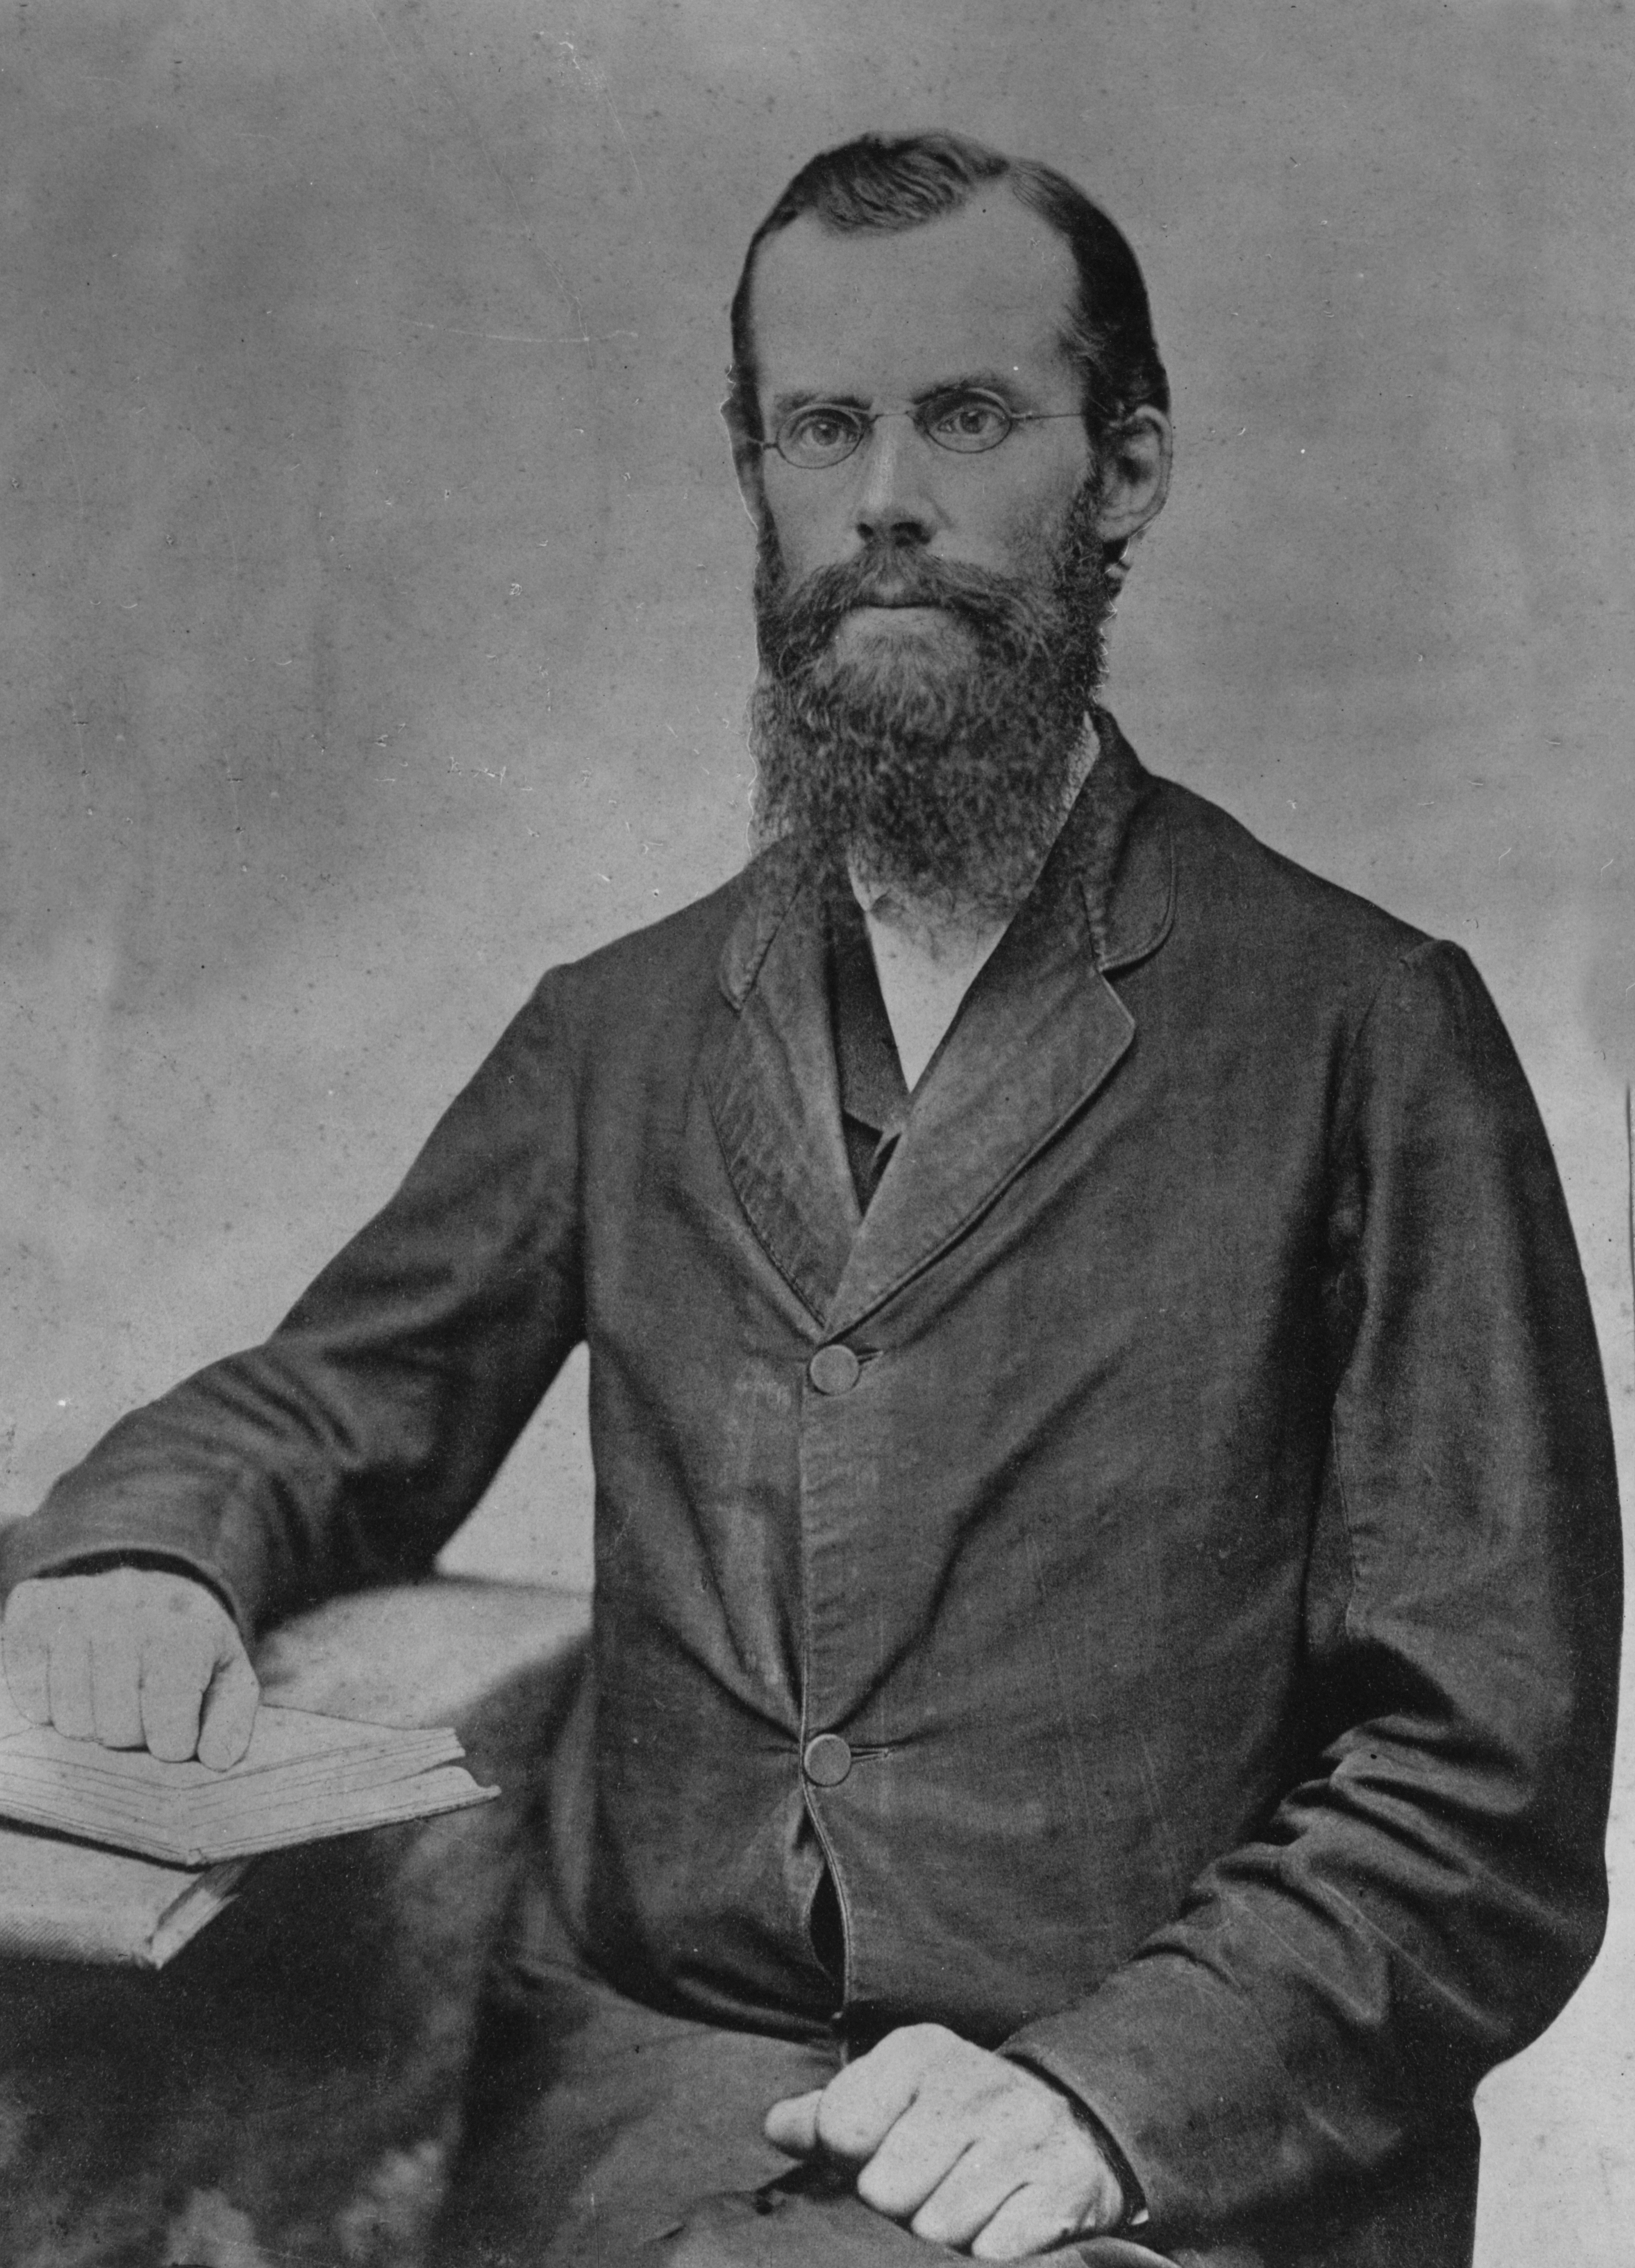
\includegraphics[width=1\linewidth]{images/john-nevins-andrews.jpg}
    \caption*{John Nevins Andrews (1829-1883)}
    \label{fig:j-n-andrews}
\end{figure}


\begin{figure}[hp]
    \centering
    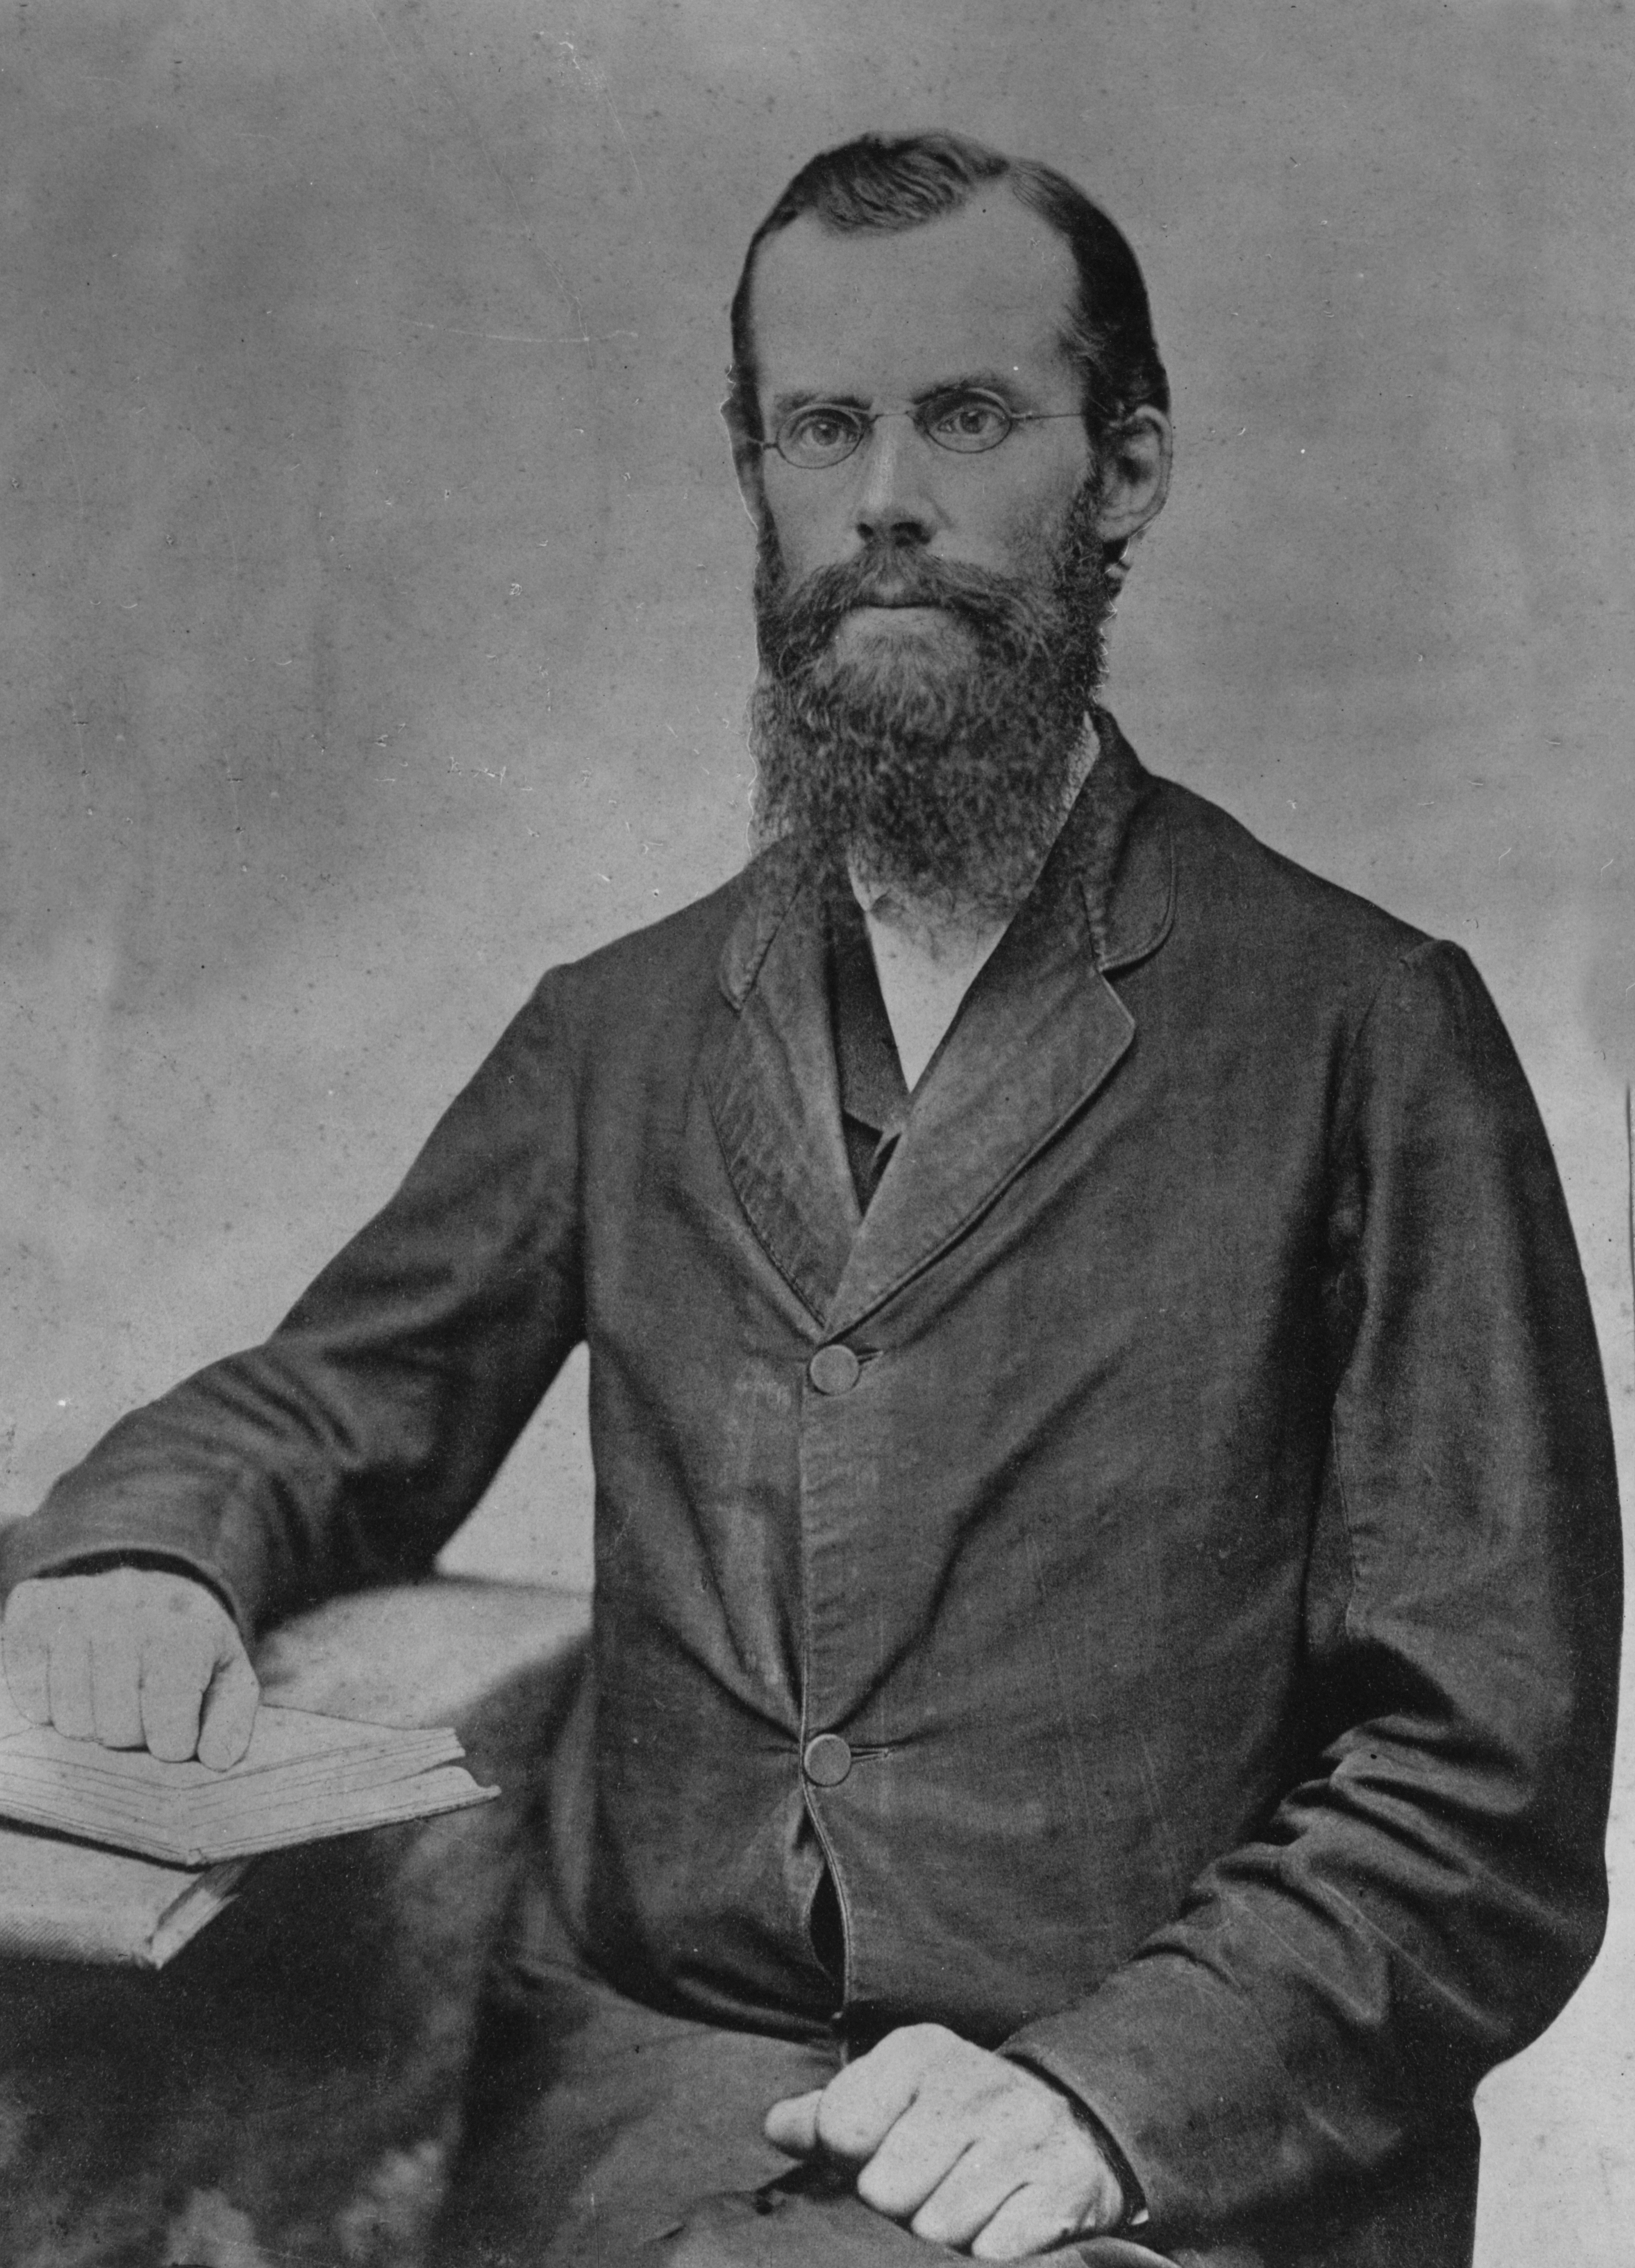
\includegraphics[width=1\linewidth]{images/john-nevins-andrews.jpg}
    \caption*{جون نيفينز أندروز (1829-1883)}
    \label{fig:j-n-andrews}
\end{figure}


J. N. Andrews said, \others{\textbf{The doctrine of the Trinity which was established in the church by the council of Nicea, A. D. 325}. \textbf{This doctrine \underline{destroys the personality of God, and his Son Jesus Christ our Lord}}...}[John. N. Andrews, The Advent Review and Sabbath Herald, March 6, 1855, p. 185][http://documents.adventistarchives.org/Periodicals/RH/RH18550306-V06-24.pdf]


قال ج. ن. أندروز، \others{\textbf{إن عقيدة الثالوث التي تأسست في الكنيسة بواسطة مجمع نيقية عام 325 م}. \textbf{هذه العقيدة \underline{تدمر شخصانية الله، وابنه يسوع المسيح ربنا}}...}[John. N. Andrews, The Advent Review and Sabbath Herald, March 6, 1855, p. 185][http://documents.adventistarchives.org/Periodicals/RH/RH18550306-V06-24.pdf]


In the context of the trinitarian understanding of the \emcap{personality of God}, it is safe to say that the \emcap{personality of God}, or the quality or state of God being a person, in any understanding of Trinity doctrine is a mystery. The problem is that there is no clear view of who is that \textit{one God} who is a person? The underlying claim is made that God is One yet Three, or One in Three; yes, God is a person, and He is one, yet simultaneously He is three persons. This view can never hold any clear perception of the \emcap{personality of God}. Also, it will deny the clearest testimony of the Scriptures that the one God is the Father, and that Christ is truly His only begotten Son. Most trinitarian brothers would agree that Christ is a real and definite being but if a trinitarian were to accept the Father as a real and definite Being, he would also need to accept the Holy Spirit as a real and definite being, thus denying the Holy Spirit as being a \textit{spirit}, the means by which the Father and Son are omnipresent. Conversely, if a trinitarian accepted the Holy Spirit to be a literal spirit, having no body nor form, then he would deny the Father to be a real, definite being. In conversation over the quality or state of God being a person, there is never a clear view of the matter with promoters of the Trinity doctrine; it is subterfuge. \textit{‘Subterfuges’} is a word Sister White used to describe the deception by artifice or stratagem in order to conceal, escape, or evade\footnote{\href{https://www.merriam-webster.com/dictionary/subterfuges}{The Merriam-Webster, ‘subterfuges’} - “\textit{deception by artifice or stratagem in order to conceal, escape, or evade}”} the truth; in other words, something that you cannot grab by head or tail. This is the primary reason Sister White did not engage in the Trinity discussion that would come up in the Seventh-day Adventist Church.


في سياق الفهم الثالوثي لـ \emcap{شخصانية الله}، من الآمن القول إن \emcap{شخصانية الله}، أو الصفة أو الحالة التي يكون بها الله شخصًا، في أي فهم لعقيدة الثالوث هي لغز. المشكلة هي أنه لا توجد رؤية واضحة لمن هو \textit{الإله الواحد} الذي هو شخص؟ الادعاء الأساسي هو أن الله واحد ولكنه ثلاثة، أو واحد في ثلاثة؛ نعم، الله شخص، وهو واحد، ولكنه في نفس الوقت ثلاثة أشخاص. هذه النظرة لا يمكن أن تحمل أي تصور واضح لـ \emcap{شخصانية الله}. كما أنها ستنكر أوضح شهادة للكتاب المقدس بأن الإله الواحد هو الآب، وأن المسيح هو حقًا ابنه الوحيد المولود. معظم الإخوة الثالوثيين سيوافقون على أن المسيح هو كائن حقيقي ومحدد، ولكن إذا قبل الثالوثي الآب ككائن حقيقي ومحدد، فسيحتاج أيضًا إلى قبول الروح القدس ككائن حقيقي ومحدد، وبالتالي إنكار الروح القدس باعتباره \textit{روحًا}، الوسيلة التي يكون بها الآب والابن حاضرين في كل مكان. وعلى العكس من ذلك، إذا قبل الثالوثي أن الروح القدس هو روح حرفي، ليس له جسد ولا شكل، فإنه سينكر أن الآب كائن حقيقي ومحدد. في المحادثة حول الصفة أو الحالة التي يكون بها الله شخصًا، لا توجد أبدًا رؤية واضحة للمسألة مع مروجي عقيدة الثالوث؛ إنها حيلة. \textit{‘الحيل’} هي كلمة استخدمتها الأخت وايت لوصف الخداع بالحيلة أو المكيدة من أجل إخفاء الحقيقة أو الهروب منها أو تجنبها\footnote{\href{https://www.merriam-webster.com/dictionary/subterfuges}{The Merriam-Webster, ‘subterfuges’} - “\textit{الخداع بالحيلة أو المكيدة من أجل إخفاء الحقيقة أو الهروب منها أو تجنبها}”} ؛ بمعنى آخر، شيء لا يمكنك الإمساك به من رأسه أو ذيله. هذا هو السبب الرئيسي لعدم مشاركة الأخت وايت في مناقشة الثالوث التي ستظهر في كنيسة الأدفنتست السبتيين.


\egw{I was cautioned not to enter into controversy \textbf{regarding the question} that \textbf{\underline{will come up}} over \textbf{these things, because controversy \underline{might lead men to resort to subterfuges, and their minds would be led away from the truth of the Word of God to assumption and guesswork}}. \textbf{The more that fanciful theories are discussed, the \underline{less men will know of God and of the truth that sanctifies the soul}}.}[Lt232-1903.41; 1903][https://egwwritings.org/read?panels=p10197.50]


\egw{لقد حُذرت من الدخول في جدال \textbf{بخصوص المسألة} التي \textbf{\underline{ستظهر}} حول \textbf{هذه الأمور، لأن الجدال \underline{قد يدفع الناس إلى اللجوء إلى الحيل، وستبتعد عقولهم عن حقيقة كلمة الله إلى الافتراض والتخمين}}. \textbf{كلما نوقشت النظريات الخيالية أكثر، \underline{قل ما يعرفه الناس عن الله وعن الحقيقة التي تقدس النفس}}.}[Lt232-1903.41; 1903][https://egwwritings.org/read?panels=p10197.50]


When we read the works of Seventh-day Adventist pioneers on the \emcap{personality of God}, we see that they did not fall into the Trinity trap. Their non-trinitarian views of God were not due to ignorance, but a knowledge of the truth on the \emcap{personality of God}. They were of keen and noble intellect, understanding the thin line between the truth and error. Their understanding of the \emcap{personality of God} is balanced and solid, strongly supported by the plain and simple “\textit{thus says the Lord}”.


عندما نقرأ أعمال رواد الأدفنتست السبتيين حول \emcap{شخصانية الله}، نرى أنهم لم يقعوا في فخ الثالوث. آراؤهم غير الثالوثية عن الله لم تكن بسبب الجهل، بل بسبب معرفة الحقيقة حول \emcap{شخصانية الله}. كانوا ذوي ذكاء نبيل وحاد، يفهمون الخط الرفيع بين الحقيقة والخطأ. فهمهم لـ \emcap{شخصانية الله} متوازن وصلب، مدعوم بقوة بـ “\textit{هكذا يقول الرب}” البسيط والواضح.


Many Adventists today accept the Trinity doctrine because Ellen White supposedly accepted it and promoted it. This is far from the truth and such a conclusion is predicated on lacking knowledge of the Spirit of Prophecy. If anyone was acquainted with the beliefs of Sister White, it was her husband James White. Here is what he has to say about the writings of his wife:


يقبل العديد من الأدفنتست اليوم عقيدة الثالوث لأن إلين وايت يُفترض أنها قبلتها وروجت لها. هذا بعيد عن الحقيقة ومثل هذا الاستنتاج مبني على نقص المعرفة بروح النبوة. إذا كان هناك شخص على دراية بمعتقدات الأخت وايت، فهو زوجها جيمس وايت. إليكم ما يقوله عن كتابات زوجته:


\others{\textbf{We invite all to compare the testimonies of the Holy Spirit through Mrs. W., with the word of God}. \textbf{And in this we do not invite you to compare them \underline{with your creed}}. That is quite another thing. \textbf{\underline{The trinitarian may compare them with his creed, and because they do not agree with it, condemn them}}. The observer of Sunday, or the man who holds eternal torment an important truth, and the minister that sprinkles infants, may each condemn the testimonies’ of Mrs. W. because they do not agree with their peculiar views. And a hundred more, each holding different views, may come to the same conclusion. \textbf{But their genuineness can never be tested in this way}.}[James S. White, The Advent Review, and Herald of the Sabbath, June 13, 1871][https://documents.adventistarchives.org/Periodicals/RH/RH18710613-V37-26.pdf]


\others{\textbf{ندعو الجميع لمقارنة شهادات الروح القدس من خلال السيدة وايت، مع كلمة الله}. \textbf{وفي هذا لا ندعوكم لمقارنتها \underline{مع عقيدتكم}}. هذا شيء آخر تمامًا. \textbf{\underline{قد يقارنها الثالوثي مع عقيدته، ولأنها لا تتفق معها، يدينها}}. مراقب يوم الأحد، أو الشخص الذي يعتبر العذاب الأبدي حقيقة مهمة، والوزير الذي يرش الأطفال، قد يدين كل منهم شهادات السيدة وايت لأنها لا تتفق مع وجهات نظرهم الخاصة. ومائة آخرون، كل منهم يحمل وجهات نظر مختلفة، قد يصلون إلى نفس الاستنتاج. \textbf{لكن صحتها لا يمكن اختبارها أبدًا بهذه الطريقة}.}[James S. White, The Advent Review, and Herald of the Sabbath, June 13, 1871][https://documents.adventistarchives.org/Periodicals/RH/RH18710613-V37-26.pdf]


James White was the closest associate of Ellen White, the person who was one with her in God’s uplifting of the Seventh-day Adventist Church. We have a clear and direct testimony from him that Ellen White’s writings are not trinitarian. Today, scholars put a false narrative that Ellen White grew in her understanding of the Trinity doctrine, and eventually accepted and preached it. But we see that Ellen White did not change her standpoint on the \emcap{personality of God} nor did she adhere to the Trinity doctrine. She was unambiguous in her claim that she never did. When the Kellogg crisis came over the \emcap{personality of God}, she remained firm in her view, just as all early Seventh-day Adventist pioneers did—and her dealings with Dr. Kellogg prove that. It is true, the Trinity doctrine \textit{cannot be accepted by those who are loyal to the faith and to the principles that have withstood all the opposition of satanic influences}.\footnote{\egw{Patchwork theories cannot be accepted by those who are loyal to the faith and to the principles that have withstood all the opposition of satanic influences}[Lt253-1903.28; 1903][https://egwwritings.org/read?panels=p14068.9980036]} Today’s official narrative that Ellen White was teaching the Trinity echoes Dr. Kellogg’s claim that the Living Temple taught the same thing as Ellen White. \egwinline{\textbf{But God forbid that this sentiment should prevail}.}[SpTB02 53.3; 1904][https://egwwritings.org/read?panels=p417.272]


كان جيمس وايت أقرب شريك لإلين وايت، الشخص الذي كان واحدًا معها في رفع الله لكنيسة الأدفنتست السبتيين. لدينا شهادة واضحة ومباشرة منه بأن كتابات إلين وايت ليست ثالوثية. اليوم، يضع العلماء رواية كاذبة مفادها أن إلين وايت نمت في فهمها لعقيدة الثالوث، وقبلتها وبشرت بها في النهاية. لكننا نرى أن إلين وايت لم تغير موقفها من \emcap{شخصانية الله} ولم تلتزم بعقيدة الثالوث. كانت واضحة في ادعائها بأنها لم تفعل ذلك أبدًا. عندما جاءت أزمة كيلوغ حول \emcap{شخصانية الله}، ظلت ثابتة في وجهة نظرها، تمامًا كما فعل جميع رواد الأدفنتست السبتيين الأوائل - وتعاملها مع الدكتور كيلوغ يثبت ذلك. صحيح أن عقيدة الثالوث \textit{لا يمكن قبولها من قبل أولئك المخلصين للإيمان وللمبادئ التي صمدت أمام كل معارضة التأثيرات الشيطانية}.\footnote{\egw{نظريات الترقيع لا يمكن قبولها من قبل أولئك المخلصين للإيمان وللمبادئ التي صمدت أمام كل معارضة التأثيرات الشيطانية}[Lt253-1903.28; 1903][https://egwwritings.org/read?panels=p14068.9980036]} الرواية الرسمية اليوم بأن إلين وايت كانت تعلّم الثالوث تردد صدى ادعاء الدكتور كيلوغ بأن كتاب ذا ليفينغ تمبل علّم نفس الشيء الذي علّمته إلين وايت. \egwinline{\textbf{لكن الله يمنع أن يسود هذا الرأي}.}[SpTB02 53.3; 1904][https://egwwritings.org/read?panels=p417.272]


% Adventist pioneers and the Trinity doctrine

\begin{titledpoem}
    \stanza{
        The pioneers stood firm against the Trinity's sway, \\
        Their testimony clear as the light of day. \\
        They saw how this doctrine did subtly disguise, \\
        What Scripture reveals to discerning eyes.
    }

    \stanza{
        James White declared it among "popular fables" found, \\
        A teaching that makes God's personality unsound. \\
        For Father and Son as distinct beings stand, \\
        Not merged into one as the Trinity planned.
    }

    \stanza{
        Two separate persons with purpose aligned, \\
        In spirit and action, united in mind. \\
        Just as disciples in Christ become one, \\
        Yet remain individual under God's Son.
    }

    \stanza{
        The Holy Spirit, God's presence divine, \\
        Not a separate being of the Godhead's design. \\
        But truly God's Spirit sent forth from above, \\
        The Father's representative, agent of love.
    }

    \stanza{
        No Scripture supports what tradition declared, \\
        When at Nicea this doctrine was shared. \\
        John seventeen shatters the trinitarian view, \\
        Revealing the Father and Son as beings true.
    }

    \stanza{
        Christ's divinity rests not in mysterious three, \\
        But in His begotten Sonship we see. \\
        The express image of His Father's face, \\
        Inheriting fullness of divine grace.
    }

    \stanza{
        The pioneers knew what the Bible made clear, \\
        That God is the Father, a Being most dear. \\
        A personal, spiritual presence on high, \\
        Omnipresent through Spirit, yet dwelling on high.
    }

    \stanza{
        So stands the truth against error's long night, \\
        Preserved by the pioneers and Sister White. \\
        Not through confusion or mystical thought, \\
        But through plain Scripture the truth has been taught.
    }
\end{titledpoem}